\section{Introduction}
\label{sec:intro}

It has long been an interesting interdisciplinary scientific challenge to 
understand the languages of animals~\cite{hockett1959animal, radick2007simian,von1974yerkish}. Dogs, who are arguably the best friends
of humans, have drawn particular attention. Learning what dogs want to 
express has broad and profound significance, such as in understanding 
biological evolution~\cite{pongracz2017modeling}, for applying their languages 
to information technology, or sometimes just for satisfying the
our curiosity.

%这里插一个引用关于“voice is one of the main communication ways of dogs"的论文
%\MY{Voice on dog is weird: vocal communication/sound production is more appropriate}
% \KZ{Should be ``vocal expression'' not
% ``vocal expression''. The latter includes gesture as well.}
Vocal expressions of dogs, being their chief means of communication, have been studied previously. Here we define vocal expressions as all the sounds that a dog can make vocally, including bark, whine, whimper, howl, huff, growl, yelp, and yip.
It has been shown that dogs can recognize the scenes and express their understandings of the outer world as well as their inner states by their voices~\cite{molnar2008classification, hantke2018my}. 
% \KZ{Rephrase: These works, however, have certain limitations on 
% their methods and datasets 
% for people to apply their results into the task of understanding dogs, 
% or in other words, match barks of dogs with their corresponding meanings.} 
The limitations of previous works are from two aspects. On the one hand, previous research treats this task as a simple 
classification problem, which means that an audio segment containing barks will be straightforwardly sent into one model to get a particular label such as emotion (happy or sad). Although the results of them have shown that dogs have consistent sound patterns for different purposes, they provided little insight into exploring whether dogs have structural languages. The potential linguistic patterns beyond the dog's vocal expressions are dramatically ignored. On the other hand, previous datasets are collected by recording the voices of dogs under certain controlled environments. Such methodology is costly in practice, and the data thus produced is limited in size and variety (as we will show later in \tabref{tab:previousdataset}). In this way, it's hard to infer the latent linguistic patterns. The patterns and semantic meanings of some environments not covered in these datasets will not be investigated as well.
%\MY{Similarly, when you describe a fact as ``limitation'', make sure that you point out why being small and less various is a limitation? }
%\MY{Why treating it as a classification problem is limited? Say it clearly that these classification studies indicate that dogs have consistent sound patterns for different purposes, however these works still provide little insight on exploring whether dogs have structural language.}


\begin{figure}[h]
\centering
\scalebox{0.3}{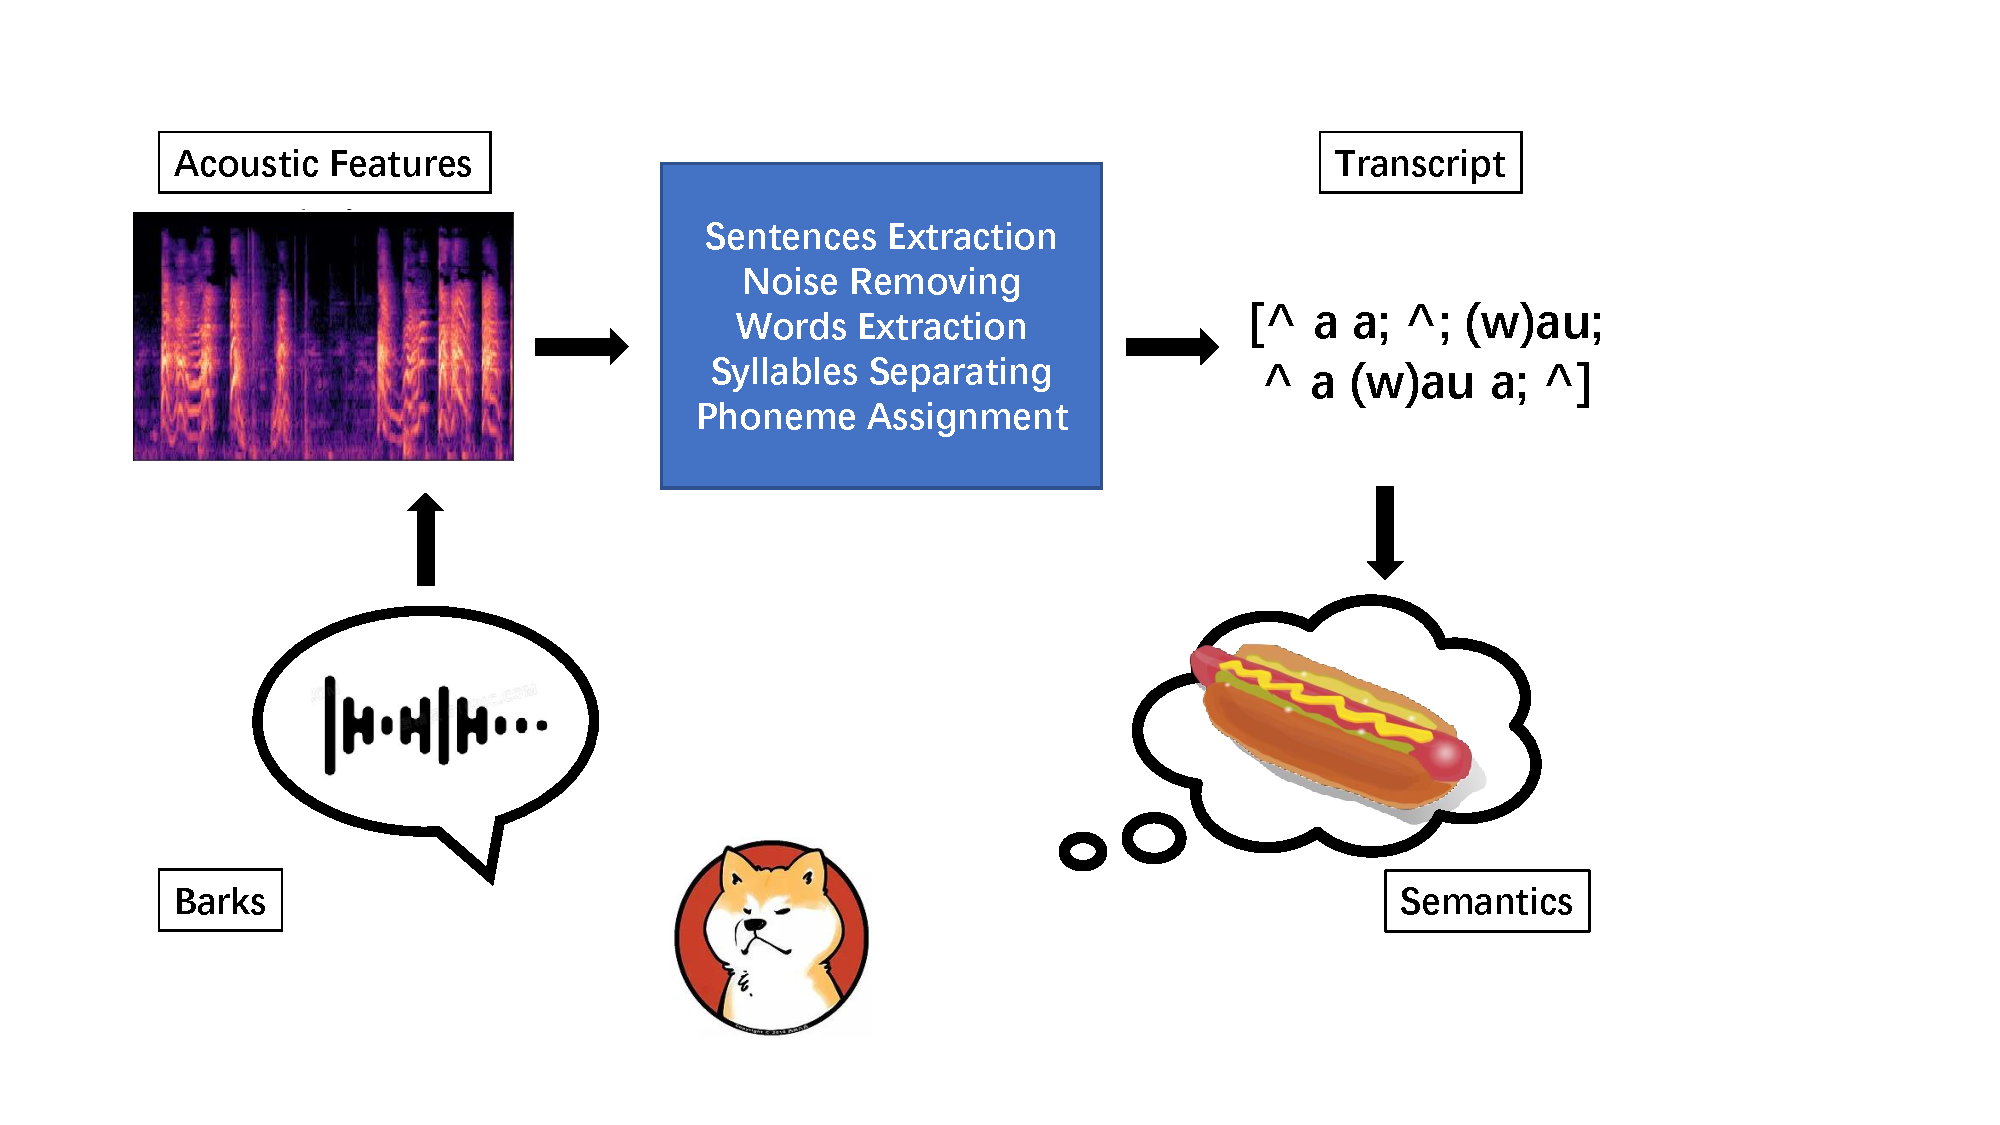
\includegraphics{intro2.pdf}}
\caption{We aim at matching the barks of dogs with its semantic meanings. In our approach, the barks of dogs will be transcribed into symbols. 
%The same example will be used in~\secref{sec:approach}.
}
\label{fig:dog}
\end{figure}
% \KZ{include an intro picture to show our aim.}

Even though it is still highly debatable whether animals, or dogs in this
case, have languages at all, in this paper, we present an approach pipeline to treat dog sounds as a kind of language, similar to human languages. 
During this process~(\figref{fig:dog}), the specific patterns found in their vocal expressions imply that their barking sounds can carry corresponding semantic meanings just as humans use fixed sound patterns to signify.
%\KZ{Rephrase this: Between the audios and meanings, 
%we can get texts as the bridge.} 
%\MY{Use present tense in intro. Can add a sentence to elaborate the first point, that if we can find specific patterns of dogs' vocial expressions, their barking sounds could carry corresponding semantic meaning just as humans use fixed sound patterns to signify. Also, why a rare human language? It's just a language, animal language}
In this paper, we present a dataset of phonetically symbolic transcripts of Shiba Inu dog barks~\footnote{Here we refer to ``barks'' in its broadest sense, which includes any vocal expressions coming from a dog.} called \textit{ShibaScript}, which ameliorates some of the aforementioned challenges. We pick Shiba Inu as the subject because it is a popular breed around the world and there are a large number of their videos on the web. Meanwhile, we provide preliminary phonetic analysis on this dataset. We believe that this work is a first step toward investigating whether dogs have sound-actuated language just as humans with speech.

%can bring much support for further research in 
%this pioneering field. \MY{Weak argument. maybe something like``To enlighten our knowledge on understanding animal languages/ a first step to investigate whether dogs have sound-actuated language just as humans with speech''}

%\KZ{I think no need to have subsections in the intro to save space.}
ShibaScript contains barks coming from 16 different Shiba Inu dogs, corresponding transcripts with timestamps of their barks, among which consistent sound patterns are found. These 16 dogs are respectively from 16 families who post these dogs' videos on YouTube. The dataset has a total length of over 4 hours of pure dog sound production, 4469 sentences, and 7761 words. There are in total 9 distinct syllables in these transcripts. 
% \MY{I think it is critical to mention that consistent sound patterns are found over these dogs/videos, cuz this is an initial yet important clue to say that whether sounds are symbolic for dogs as if for humans} Mention below: Contributions.
Note that due to the ever-evolving nature of social media, the dataset-construction methodology we propose in this paper can be applied to YouTube continuously and yields a dataset that is growing in size and variety. We believe this dataset will help with future research on canine communication as well as any general audience who are interested in learning what dogs want to express.

%\subsection*{Contributions}
Our contributions lie in three aspects: 
\begin{enumerate}
\item we introduce a reusable framework for transcribing animal voices from social media like YouTube, the framework is the first to assign phonetic symbols on dog barks as well as describe dogs' vocal communication in a formal way; 
\item we release a novel Shiba Inu voice transcription dataset~\footnote{The complete code and dataset are available at \url{https://github.com/XSiling/ShibaScript}.}, which is the first of its kind in the CL community; 
\item we present some preliminary statistical findings from this dataset. 9 consistent phonetic symbols are discovered, with phonemes/words/sentences being existent, The consistent sound patterns found over the these dogs reveal that dogs may have structural vocal communication patterns.
% \MY{Put down your main findings, e.g. 8 consistent phoneme symbols and that dogs could have structural vocal communication patterns}
\end{enumerate}
% \MY{we are the first to assign phonetic symbols on dog barks, to describe dogs' vocal communication in a formal way}

% \MY{A general comment: you need to avoid using ``it's'' ``it'', these are informal expressions and usually not used in academic writing. Just put them in full, or use present tense for it}OK, gonna fix
